\documentclass[10pt,twocolumn]{article}
\usepackage{fullpage,enumerate,amsmath,amssymb,graphicx,setspace,epstopdf,float,multirow}

\begin{document}
\title{CS 276 Programming Assignment 3 Project Report}
\author{Jiaji Hu, Xuening Liu}
\date{}
\maketitle

\section*{Task 1: Cosine Similarity}
Our parameters for task 1:
\begin{table}[H]
\centering
\begin{tabular}{|c|c|}
\hline
Parameter & value \\\hline
task1\_W\_url & 3.1\\\hline
task1\_W\_title & 5.0\\\hline
task1\_W\_body & 1.1\\\hline
task1\_W\_header & 1.6\\\hline
task1\_W\_anchor & 0.5\\\hline
body\_len\_normalization & 500\\\hline
tf\_scaling & linear\\\hline
\end{tabular}
\end{table}
The performance of our scorer is shown below:
\begin{table}[H]
\centering
\begin{tabular}{|c|c|}
\hline
Dataset & NDCG/iNDCG score \\\hline
training & 0.8671\\\hline
dev & 0.8462\\\hline
\end{tabular}
\end{table}
After extensive tuning, we figured out that tuning parameters for cosine similarity does rather little to help with performance. However, we used this task to develop our methodology for tuning parameters, which helped us a lot in the following tasks.

First of all, after some experimenting, we discovered that if we just tuned one parameter, keeping the others the same, there was often one peak ``good'' value for that parameter, so that the score was maximized. Here is an example:
\begin{figure}[H]
\centering
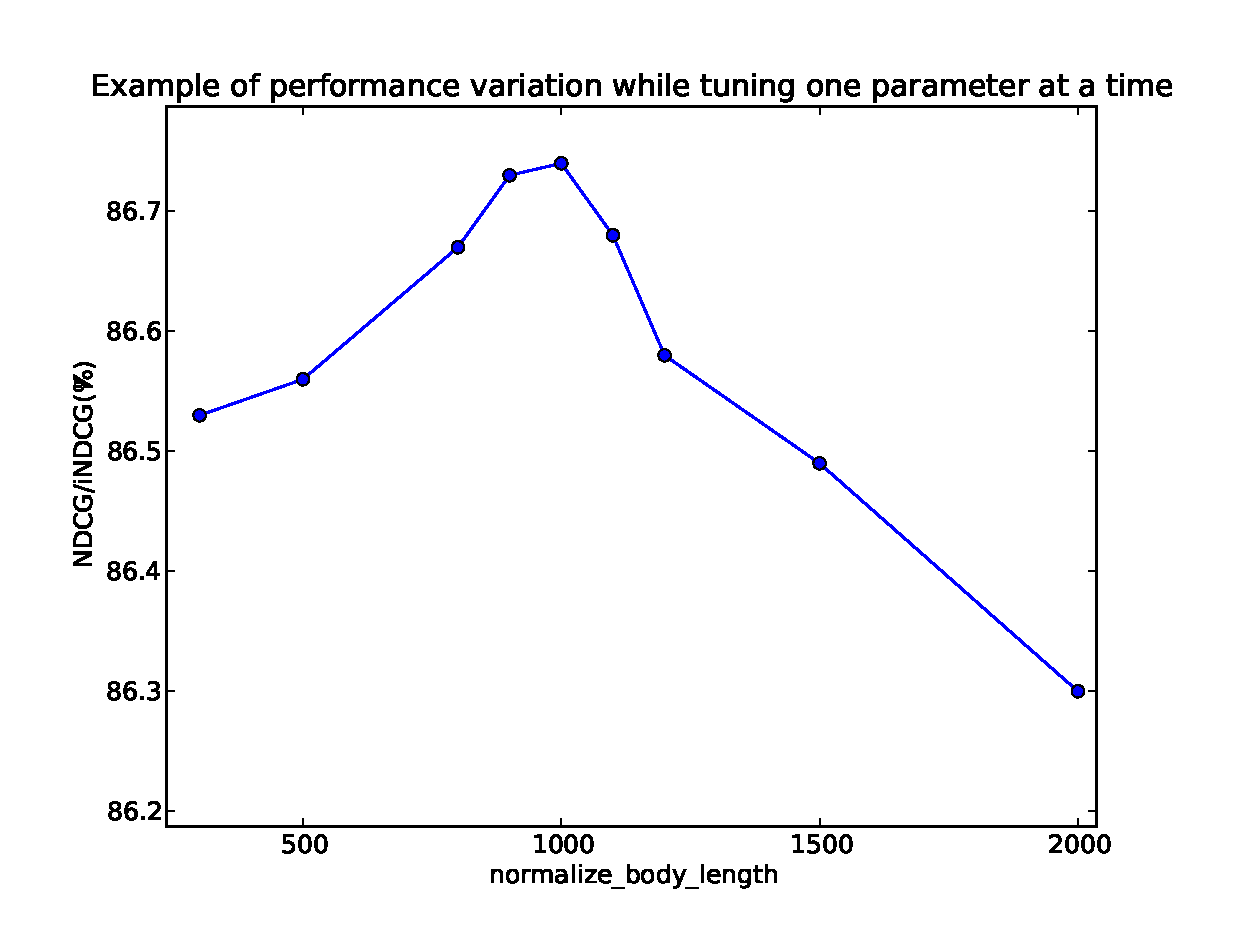
\includegraphics[width=0.7\linewidth]{fig1}
\end{figure}
It was usually the case that there is only one such peak value, and that we were able to find it by simple ``hill climbing''.

After we found the peak for one parameter, we could move on to the next parameter and find its peak value. By making a few iterations through all the parameters, we were able to more or less converge to a set a parameters that gave good performance.

The advantage to such a method is that it is simple, effective and easy to understand. It was often the case that we were able to converge to a local maximum in a few dozen tries. The results were also quite good, especially for our BM25F scorer, which ended up getting many sets of local optima above 0.888 on the training set. Last but not least, we knew what we were doing at every step, and were therefore able to gain some additional insight into the field weights.

Compare this to an exhaustive search over the parameter space (which we actually tried doing with a script) --- even with just 10 possible values per field and 6 fields, we would end up with a million data points to compute, which would take around a year. We also considered some other interesting search algorithms such as beam search, but decided that hill-climbing was easier to utilize. (Beam search, in itself, has parameters that need tuning.)

The drawback of hill climbing is that it may get stuck in local optima. We observed that since there is an ordering of which parameters get tuned first, the first ones tend to overfit the parameters that are yet to be tuned. When the time comes to tune the last parameters, little adjustment needs to be made, because the algorithm is already stuck at a local optimum. To combat this, we introduced some randomization of the ordering of parameters, and did multiple runs to find the best results.

Finally, some discussion on the reasoning behind our final parameter weights for cosine similarity, and some attempts to explain the results:

First, the choice to use linear or sublinear scaling for term frequencies is an important factor. Using sublinear scaling will greatly lower the impact of high frequency appearances of a query term in a field. If we look closely at the data, we realize that this would mostly affect the \texttt{body} and \texttt{anchor} fields, since these two fields often have high frequency appearances of query terms. On a high level, this choice is a design choice of how much emphasis we want to put on the fact that a query term appears many times in the same field of a document. In practice, linear scaling gave better performance on the cosine similarity scorer, so that was our choice.

Next, we discuss the weights for the five fields. Intuitively, higher weights should be given to fields that are good predictors of a document's relevance to a query. In practice, we realized that because we were not doing good normalization (but instead just dividing the same number for all the fields), we also needed to take into account the fact that some fields were more likely to gain higher counts of the query terms than others.

Before the results of our parameter tuning came out, we thought that the \text{title} and \text{anchor} fields were the most important indicators, and therefore should have the highest weights. We were right about \text{title}, but very wrong about \text{anchor}. The following is a list of the field weights and some explanation.
\begin{enumerate}[(a)]
\item \texttt{task1\_W\_url}

\texttt{URL} got a high weight of 3.1. This may be because query terms don't always appear in the URL, but when they do, they are great indicators of the document's relevance.
\item \texttt{task1\_W\_title}

As expected, \texttt{Title} got the highest weight, 5.0. It follows intuition that having the query appear in the page title indicates high relevance. 
\item \texttt{task1\_W\_body}

The \texttt{body} field got a weight of 1.1. Note that this field often contains a high number of occurrences of query terms. Since we are not using sublinear scaling, this has a even larger impact on the document's score. To prevent the influence from overshadowing input from the other fields, the weight for the body field cannot be too high.
\item \texttt{task1\_W\_header}

We assigned a weight of 1.6 to the \texttt{header} field. However, we note that there are other sets of high-performing parameters that have the weight for this field to be higher. We concluded that the header field is not such a high-impact field as \texttt{title}, due to its content being not as indicative.
\item \texttt{task1\_W\_anchor}

We were surprised to find the best weight for the \texttt{anchor} field to be as low as 0.5. Upon further discussion, we attribute this to the fact that this field often has a high number of query term occurrences, so the weights need to be lower to normalize for that. Also, having a large number of anchors pointing to a page means the page is likely a homepage or hub (e.g. \texttt{www.stanford.edu}), which may be too general and therefore may not satisfy a specific information need.
\end{enumerate}

Lastly, we discuss body length smoothing. Since we are using length normalization, this value directly affects the score of a document. More smoothing would mean less harsh normalization for longer documents compared to the shorter ones. From our experiments, the best value to be used for smoothing the body lengths was found to be 500.

\section*{Task 2: BM25F}
Our parameter weights for task 2:
\begin{table}[H]
\centering
\begin{tabular}{|c|c|}
\hline
Parameter & value \\\hline
task2\_W\_url & 3.3\\\hline
task2\_W\_title & 5.2\\\hline
task2\_W\_body & 0.9\\\hline
task2\_W\_header & 2.85\\\hline
task2\_W\_anchor & 3.45\\\hline
task2\_B\_url & 0.0\\\hline
task2\_B\_title & 0.2\\\hline
task2\_B\_body & 0.8\\\hline
task2\_B\_header & 0.5\\\hline
task2\_B\_anchor & 0.0\\\hline
tf\_scaling & sublinear\\\hline
K1 & 4.9\\\hline
$\lambda$ & 3.25\\\hline
$\lambda'$ & 0.05\\\hline
$\lambda''$ & 0.1\\\hline
\end{tabular}
\end{table}
Where the function $V_j$ is as follows:
\begin{equation*}
V_j = \frac{1}{\lambda'+\exp({-f_j\lambda''})}
\end{equation*}

NOTE: give values for weights and discuss intuition.

What was the reasoning behind giving the weights to the url, title,
body, header and anchor fields for the three tasks? Were there any
particular properties about the documents that allowed a higher weight
to be given to one field as opposed to another?

In BM25F, in addition to the weights given to the fields, there are
8 other parameters, Burl;Btitle;Bheader;Bbody;Banchor, lambda; lambda\_prime and K1.
How do these parameters affect the ranking function?

In BM25F, why did you select a particular Vj function?

\section*{Task 3: Smallest Window}
Our parameters for task 2:
\begin{table}[H]
\centering
\begin{tabular}{|c|c|}
\hline
Parameter & value \\\hline
task2\_W\_url & 3.3\\\hline
task2\_W\_title & 5.2\\\hline
task2\_W\_body & 0.9\\\hline
task2\_W\_header & 2.85\\\hline
task2\_W\_anchor & 3.45\\\hline
task2\_B\_url & 0.0\\\hline
task2\_B\_title & 0.2\\\hline
task2\_B\_body & 0.8\\\hline
task2\_B\_header & 0.5\\\hline
task2\_B\_anchor & 0.0\\\hline
tf\_scaling & sublinear\\\hline
K1 & 4.9\\\hline
$\lambda$ & 3.25\\\hline
$\lambda'$ & 0.05\\\hline
$\lambda''$ & 0.1\\\hline
B & \\\hline

\end{tabular}
\end{table}
Where the page rank function $V_j$ is as follows:
\begin{equation*}
V_j = \frac{1}{\lambda'+\exp({-f_j\lambda''})}
\end{equation*}
And smallest window boosting function is as follows:
\begin{equation*}
score = score \times [1+(B-1)\exp(query\_len-win\_size)]
\end{equation*}

NOTE: give values for weights and discuss intuition.
What was the reasoning behind giving the weights to the url, title,
body, header and anchor fields for the three tasks? Were there any
particular properties about the documents that allowed a higher weight
to be given to one field as opposed to another?

For a function that includes the smallest window as one component,
how does varying B and the boost function change the performance
of the ranking algorithm?

\section*{Task 4: Extra Credit}

\section{Summary Analysis}
NOTE: compare ranking functions

What was the reasoning behind giving the weights to the url, title,
body, header and anchor fields for the three tasks? Were there any
particular properties about the documents that allowed a higher weight
to be given to one eld as opposed to another?

What other metrics, not used in this assignment, could be used to
get a better scoring function from the document? The metrics could
either be static (query-independent, e.g. document length) or dynamic
(query-dependent, e.g. smallest window).

\section{ideas}
\begin{enumerate}
\item 
Tuning weights of fields: Increase one weight at a time, monitor change in performance.
\item
NOTE: report stats on both training and dev data!
\item 
experiment with stemming? experiment with other smoothing strategies?(cosine body length).
\end{enumerate}

\end{document}